\documentclass[a4paper,12pt]{scrartcl} 

\usepackage{hyperref}
\usepackage[german]{babel} 
\usepackage[utf8]{inputenc}
\usepackage{setspace}
\usepackage{cite}
\usepackage{graphicx}
\usepackage{array}
\setlength{\parindent}{0em}
\usepackage{booktabs}
\usepackage{amsmath}
\usepackage{amsfonts}
\usepackage{amssymb}
\usepackage{caption}
\usepackage[paper=a4paper,left=30mm,right=30mm,top=30mm,bottom=30mm]{geometry} 
\usepackage[nottoc, numbib]{tocbibind}
\usepackage{CJKutf8}
\usepackage[T3,OT2,T1]{fontenc} 
\usepackage[noenc]{tipa}
\usepackage{listings}
\usepackage{fancybox}
\usepackage{multirow}
\usepackage{cprotect}
\usepackage{enumerate}
\usepackage[usenames,dvipsnames]{xcolor}
\usepackage{setspace}
\usepackage{url}

%Abstand der Fussnoten
\deffootnote{1em}{1em}{\textsuperscript{\thefootnotemark\ }}

\newcommand{\rr}{\raggedright}
\setcounter{secnumdepth}{3}

\newcolumntype{P}[1]{>{\raggedright\arraybackslash}p{#1}}
\makeatletter
\newcolumntype{F}[1]{>{\raggedright\arraybackslash\@minipagetrue\flushemize}p{#1}<{\endflushemize}}
\makeatother

\newenvironment{flushemize}{%
    % You should put this outside the `list`. The new environment will make them local anyway:
    \setlength{\itemsep}{0pt}%
    \setlength{\parskip}{0.1pt}%
    \setlength{\parsep}{0.1pt}%
    \setlength{\partopsep}{0.1pt}%
    \setlength{\topsep}{0pt}%
    \setlength{\leftmargin}{6pt}%
    % Use \list ... \endlist instead of \begin{list} ... \end{list} inside another environment
    \list{$\bullet$}\unskip}
    {\endlist}

\begin{document}


%Beginn der Titelseite
\begin{titlepage}
\begin{small}
\vfill {Ruprecht-Karls-Universität Heidelberg\\ 
Institut für Computerlinguistik\\ 
Sommersemester 2015\\
Advanced Programming (P III) \\
Shigehiko Schamoni}
\end{small}


\begin{center}
\begin{Large}
\vfill {\textsf{\textbf{
Ein parallelisiertes Sprachmodell
}}}
\end{Large}
\end{center}

\begin{small}
\vfill <Daten>
\today
\end{small}

\end{titlepage}
%Ende der Titelseite


%Inhaltsverzeichnis (aktualisiert sich erst nach dem zweiten Setzen)
\tableofcontents
\newpage
\thispagestyle{empty}

\section{Einleitung}

    Sprachmodelle sind ein etabliertes und oft verwendetes Mittel innerhalb der Computerlinguistik, z.B. bei der maschinellen Übersetzung, bei Spracherkennung und Part-of-Speech Tagging. \\
    So einfach das Grundprinzip dieser Modelle so ist, so schwierig kann die Implementierung bei einer steigenden Menge von Eingabedaten daten, da bestimmte Datenstrukturen ab für mehrere hundertausend Einträge schlichtweg nicht geeignet sind und die Laufzeiten bestimmter Rechen- bzw. Lade- oder Speichervorgänge nicht mehr praktikabel werden. \\ \\
    Deswegen erscheint es sinnvoll, dieses Problem durch das gleichzeitige Bearbeiten mehrerer Teilprobleme zu umgehen und die Gesamtdauer der Programmausführung zu verringern. Ein dahingehender Versuch soll in den folgenden Kapiteln dargstellt, erläutert und evaluiert werden.

\section{Zielsetzung}

    Das Ziel dieses Projekts ist es, ein Sprachmodell zu implementieren und dies an bestimmten Punkten sinnvoll mithilfe verschiedener Techniken zu parallelisieren, um es beschleunigen. Darüber hinaus sollen an diesen Punkten auch noch einige Experimente durchgeführt werden, um zu ermitteln, welche Konstellation von Parametern die besten Ergebnisse liefert. \\

    Es wurden folgende Punkte zur Optimierung ausgewählt:
    \begin{itemize}
        \item Zählen von Wortfrequenzen im Korpus
        \item Laden gespeicherter Daten
        \item Berechnung von \emph{n}-gram-Wahrscheinlichkeiten
        \item Evaluation des Sprachmodells gegen einen Korpus
    \end{itemize}

    In den folgenden Kapiteln sollen zuerst die verwendeten Ressourcen vorgestellt werden; anschließend wird jedem der oben genannten Punkte ein eigener Teil gewidmet, in welchem jeweils die grundsätzliche Idee, die konkrete Implementierung und die aus Versuchen resultierenden Ergebnisse erläutert werden sollen.

\section{Ressourcen}

    In diesem Kapitel werden die wichtigsten in dieser Projektarbeit gebrauchten Ressourcen näher dargestellt.

    \subsection{Wikipedia als Korpus}

    Die Online-Enzyklopädie Wikipedia weist in ihrer deutschsprachigen Version mittlerweile über 1,858 Millionen Artikel\footnote{Stand: Ende September 2015.} auf. Darum und wegen der leichten Erhältlichkeit ihrer Daten stellt sie einen in computerlinguistischen Arbeiten beliebten Korpus dar. \\
    Für diese Arbeit wurde ein XML-Dump der gesamten deutschen Wikipedia (nur Artikel ohne Diskussionen etc.) verwendet, der anschließend durch ein Python-Script in ein einfaches Text-Dokument umgewandelt wurde. Da wurden auch Satzfanfangs- (\emph{<s>}) und Satzendetags (\emph{</s>}) eingefügt\footnote{Da das Script recht naiv arbeitet, sind diese Tags nicht immer ganz richtig gesetzt. Da dieses Projekt den Fokus auch eher auf den Aufbau des Sprachmodells legt, ist dies zu vernachlässigen.}. Nach diesem Verarbeitungsschritt ergeben sich insgesamt ungefähr 14,2 Millionen Sätze mit x Tokens und y Types. \\
    Die Daten werden anschließend in ein Trainings-, ein Development- und ein Testset im Verhältnis von 60 \% - 20 \% - 20 \% aufgeteilt.

    \subsection{Hadoop \& MapReduce}

    Hadoop ist eine von Apache entwickelte Open-Source Bibliothek zum leicht skalierbaren Prozessieren großer Datenmengen\footnote{Online erreichbar unter: https://hadoop.apache.org (Zuletzt abgerufen am 29.09.15)}. Darunter befindet sich auch Hadoop MapReduce, welches die gleichnamige Parallelisierungstechnik bereitstellt. \\
    MapReduce besteht aus mehreren Operationsschritten, darunter die namensgebenden \emph{Map} und \emph{Reduce}-Schritte. Bei Map wird eine Operation auf einer Eingabe ausgeführt und zwischengespeichert, bevor sie von der \emph{Shuffle}-Funktion auf verschieden \emph{Reducer} verteilt werden, die als Summierer fungieren. Die Parallelität dieser Vorgehens besteht darin, dass gleichzeitig mehrere Map und Reduce Operationen ausgeführt werden können. 

\section{Frequenzzählung}

    \subsection{Vorgehen}

    Im Kapitel ``Hadoop \& MapReduce'' wurde bereits das Grundprinzip dieser Programmiertechnik erklärt. MapReduce lässt sich dabei sehr einfach auf die Wortfrequenzzählung anwenden (eines Demoklasse {\tt WordCount.java} ist in der Apache-Bibliothek sogar bereits vorhanden), wobei die Mapper den Input lesen und dabei das Wort und seine dazugehörige Frequenz (eins) emittieren. Die Shuffle-Funktion weist dann gleiche Wörter einem Reducer zu, der die Frequenzen summiert. \\
    Optimierungsmöglichkeiten dieses Prozesses bestehen an mehreren Punkten:
    \begin{itemize}
        \item Vor der Shuffle-Phase können sog. \emph{Combiner} zugeschaltet werden, die wie ein Reducer funktionieren und Frequenzen gleicher Wörter, die von ein und demselben Mapper emittiert wurden schon vorher summieren, sodass die Anzahl der Einträge schon vor dem Einsatz der Reducer verringert wird
        \item Die Funktion, die Wort-Frequenz-Paare an Reducer zuweist, kann umgeschrieben werden
        \item Die Anzahl von Mappern und Reducern kann variiert werden
    \end{itemize}

    Davor wurde allerdings die Demoklasse etwas angepasst, um auch Frequenzen für beliebige \emph{n}-gramme und nicht nur einzelne Wörter zählen zu können.

    \subsection{Experimente}

    Es wurden mehrere Versuche durchgeführt: Zum einen wurden die Programmlaufzeiten für verschiedenen \emph{n} mit und ohne Combiner gemessen, um herauszufinden, welchen Einfluss dieser auf die Gesamtdauer des Prozesses hat. Ursprünglich war außerdem geplant, eine eigene Partitionerfunktion zu entwerfen, die zipf'sche Natur der Wortfrequenzverteilung berücksichtigt und verschiende Verhältnisse von Mappern und Reducern zu testen. Dies musste allerdings u.A. aus Zeitgründen wegfallen. \\ \\

    Beim ersten Versuch wurden alle \emph{n}-gramme von eins bis fünf zehn Mal gezählt und die durchschnittliche Dauer der Ausführung ermittelt. Dies wurde jeweils mit Combiner wiederholt. In der Standardkonfiguration des verwendeten Clustern wurden dabei drei Mapper und ein Reducer eingesetzt.

    \begin{figure}[h]
        \centering
        \begin{tabular}{c|c||c|c}
            n & Combiner? & Zeit (in s) & Beschleunigung\\
            \hline
            \multirow{2}{*}{1} & \textcolor{BrickRed}{Nein} & 99,21 & \multirow{2}{*}{\textcolor{OliveGreen}{$\uparrow$ 45,55 \%}} \\
             & \textcolor{OliveGreen}{Ja} & 54,02 & \\
             \hline
            \multirow{2}{*}{2} & \textcolor{BrickRed}{Nein} & 122,40 & \multirow{2}{*}{\textcolor{OliveGreen}{$\uparrow$ 29,90 \%}} \\
             & \textcolor{OliveGreen}{Ja} & 90,70 & \\
             \hline
             \multirow{2}{*}{3} & \textcolor{BrickRed}{Nein} & 144,97 & \multirow{2}{*}{\textcolor{OliveGreen}{$\uparrow$ 12,94 \%}} \\
             & \textcolor{OliveGreen}{Ja} & 126,66 & \\
             \hline
             \multirow{2}{*}{4} & \textcolor{BrickRed}{Nein} & 163,30 & \multirow{2}{*}{\textcolor{OliveGreen}{$\uparrow$ 8,75 \%}} \\
             & \textcolor{OliveGreen}{Ja} & 149,02 & \\
             \hline
             \multirow{2}{*}{5} & \textcolor{BrickRed}{Nein} & 162,34 & \multirow{2}{*}{\textcolor{BrickRed}{$\downarrow$ -21,61 \%}} \\
             & \textcolor{OliveGreen}{Ja} & 197,42 & \\
        \end{tabular}
        \caption{Zeiten für die Ausführung des Programms für verschiedene \emph{n} mit und ohne Combiner.}
    \end{figure}

    Dabei zeigt sich eindrucksvoll, dass der Einsatz eines Combiners nicht zwangsläufig zu einem schnelleren Ergebnisführt; im Gegenteil, für 5-gramme ist dies sogar \textbf{kontraproduktiv}.\\

    Dies lässt sich folgendermaßen erklären: Da es sehr viele mehr Möglichkeiten gibt, fünf Wörter miteinander zu kombinieren, als dies für geringere \emph{n} der Fall ist, ist auch die Wahrscheinlichkeit des Vorkommends eines 5-gramms kleiner. Somit emittieren die Mapper bei dieser Größe fast nur noch einzigartige 5-gramme. Der Combiner, der dazu ausgelegt ist, die Werte häufiger Schlüssel zu kombinieren, wird nun fast vergebens angewendet und velängert den ganzen Prozess nur. \\

    Umgekehrt gilt auch das Gegenteil: Je weniger einzigartige Schlüssel vorhanden sind, desto höher ist der Effekt des Combiners, so z.B. bei Unigrammen, wo manche Wörter nach der Zipf-Verteilung sehr oft zu erwarten sind. \\
    Es ist auch möglich, in einem Durchgang alle Uni-, Bi-... \emph{n}-gramme auf einmal zu emittieren, jedoch dauert dies in Wirklichkeit wesentlich länger als jeder der Durchläufe für eine Größe summiert. \\

    Ein schon angesprochener Punkt besteht in der Anzahl von Mappern und Reducern. Die Anzahl von Mappern wird normalerweise von Hadoop selbst festgelegt: Die Anzahl richtet sich nach der Menge der Blöcke, in die die Eingabe aufgespalten wird \cite{hadoop}. Für die Anzahl von Reducern gibt es die Faustegel
    \[n_{reducer} = c_{reducer} * n_{nodes} * n_{max tasks}\]
    wobei $c_{reducer}$ eine Konstante ist, für die ein Wert zwischen 0,95 und 1,75 empfohlen wird, $n_{nodes}$ die Anzahl der Knoten und $n_{max tasks}$ die Anzahl der maximalen Tasks pro Knoten ist (ca. 1000). Nach einigen Versuchen schien sich diese Fautregel auch zu bewahrheiten, allerdings nimmt Hadoop die z.B. über {\tt job.setNumReduceTasks($\cdot$);} eingestellte Anzahl eher als Empfehlung und stellt die wirklichen Parameter nach wirklicher Auslastung ein, sodass Ergebnisse unter vergleichbaren Bedingungen nicht wirklich möglich sind.

\section{Berechnung von \emph{n}-gram Wahrscheinlichkeiten}

    \subsection{Vorgehen}

    Generell berechnet sich die Wahrscheinlichkeit eines \emph{n}-grams $w_{i-n+1},\ldots,w_i$ folgendermaßen
    \[p(w_i|w_{i-n+1},\ldots, w_{i-1}) = \frac{\#(w_{i-n+1},\ldots, w_{i-1}, w_i)}{\#(w_{i-n+1},\ldots, w_{i-1})} \]
    wobei $\#(\cdot)$ die Frequenz einer Wortfolge im Trainierungskorpus ist\cite{lm}. \\

    Die Frequenzen der \emph{n}-gramme werden eingelesen. Um die Wahrscheinlichkeit der Bigramme zu berechnen, werden Unigram- und Bigramfrequenzen eingelesen, bei Trigrammen Bigram- und Trigramfrequenzen usw. Durch dieses ``schichtweise'' einlesen werden müssen nicht alle Daten auf einmal in den Speicher geladen werden, was gerade bei höheren \emph{n} zu Problemen führen kann. \\
    Engstellen bei diesem Prozess sind:
    \begin{enumerate}[a)]
        \item Das Lesen der Indexing-Dateien
        \item Das Berechnen der Wahrscheinlichkeiten per se
    \end{enumerate}
    Beides kann auf relative einfache Art und Weise parallelisiert werden, was in den folgenden Abschnitten dargelegt wird.

    \subsection{Laden \& Speichern}

    Bevor die Wahrscheinlichkeiten errechnet werden, werden die Dateien mit den \emph{n}-gram Frequenzen in ein anderes Speicherformat konvertiert, sog. \emph{Indexings}. Dabei wird jedes Wort durch eine einzigeartige ID ersetzt, welche in einem Lexikon vermerkt wird. Somit ist die Speicherung der Dateien effizienter (nur Zahlen statt den ganzen Worten speichern zu müssen benötigt wesentlich weniger Speicherplatz und zahlt sich gerade bei höheren \emph{n} aus) und die Verarbeitung ein wenig schneller, da in manchen Schritten nur Zifferen und nicht Strings miteinander verglichen werden müssen. \\
    Dennoch dauert z.B. bei 4- oder 5-grammen das Einlesen ziemlich lange, da sich mit jedem Schritt die Anzahl der Einträge vervielfacht (siehe Abbildung x.), weshalb sich Parallelisierung umso mehr anbietet. In diesem Beispiel lesen einfach mehrere Threads gleichzeitig an einer Datei\footnote{Bei der {\tt BufferedReader}-Implementation von Java kommt es dazu erstaunlicherweise nicht zu Zeilenduplikaten.}.)

    \begin{figure}[h]
        \begin{minipage}[t]{0.35\textwidth}
            \centering
            \begin{tabular}{c|c}
                n & Anzahl (in Mio.) \\
                \hline \hline
                1 & 1,2372 \\
                \hline
                2 & 1,5793 \\
                \hline
                3 & 3,2014 \\
                \hline
                4 & 39,6832 \\
                \hline
                5 & 42,8007 \\
            \end{tabular}
        \end{minipage}
        \begin{minipage}{0.65\textwidth}
            \centering
            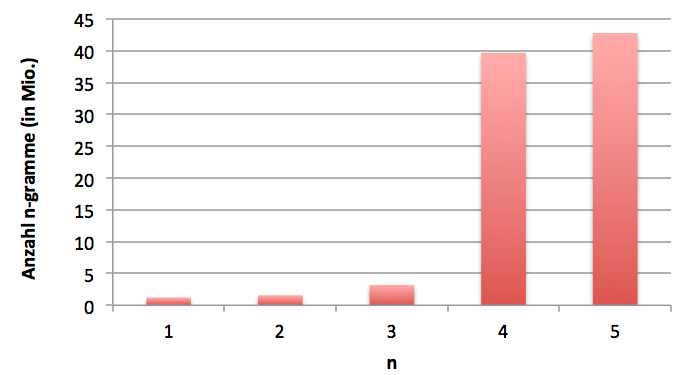
\includegraphics[width=\textwidth]{./img/ngrams.png}
        \end{minipage}
        \caption{Anzahl der einzigartigen \emph{n}-gramme im vollen Korpus. Eigene Darstellung.}
    \end{figure}

    Bei den Indexings wurde allerdings auch noch mit dem Format experimentiert, existieren neben der normalen Version auch noch zwei Varianten, bei denen sowohl die IDs der Wörter als auch das gespeicherte Ergebnis vorher in binär oder hexadezimal umgewandelt wurden. Zudem wurde getestet, wie sich das Komprimieren der Speicherdatei auf die Ladegeschwindigkeit auswirkt (auf den Speicherbedarf hat dies natürlich einen äußerst positiven Effekt).

    \begin{figure}[h]
        \centering
        \begin{tabular}{c||c|c|c}
            Indexing & Komprimiert? & Parallel? & Zeit (in s) \\
            \hline \hline
            \multirow{4}{*}{Standard} & \textcolor{BrickRed}{Nein} & \multirow{2}{*}{\textcolor{BrickRed}{Nein}} & 3,56 \\
            & \textcolor{OliveGreen}{Ja} & & 5,36 \\ \cline{2-3}
            & \textcolor{BrickRed}{Nein} & \multirow{2}{*}{\textcolor{OliveGreen}{Ja}} & \textbf{2,8} \\
            & \textcolor{OliveGreen}{Ja} & & 4,96 \\
            \hline
            \multirow{4}{*}{Binär} & \textcolor{BrickRed}{Nein} & \multirow{2}{*}{\textcolor{BrickRed}{Nein}} & $2,0 * 10^{-7}$\\
            & \textcolor{OliveGreen}{Ja} & & $2,05 * 10^{-7}$ \\ \cline{2-3}
            & \textcolor{BrickRed}{Nein} & \multirow{2}{*}{\textcolor{OliveGreen}{Ja}} & $2,73 * 10^{-7}$ \\
            & \textcolor{OliveGreen}{Ja} & & $\mathbf{1,75 * 10^{-7}}$ \\
            \hline
            \multirow{4}{*}{Hexadezimal} & \textcolor{BrickRed}{Nein} & \multirow{2}{*}{\textcolor{BrickRed}{Nein}} & 3,59 \\
            & \textcolor{OliveGreen}{Ja} & & 6,07 \\ \cline{2-3}
            & \textcolor{BrickRed}{Nein} & \multirow{2}{*}{\textcolor{OliveGreen}{Ja}} & \textbf{3,46} \\
            & \textcolor{OliveGreen}{Ja} & & 5,0 \\
        \end{tabular}
        \caption{Parallele und sequentielle Ladezeiten von rohen und komprimierten Indexings. Ausgeführt mit vier Threads auf einer Maschine mit zwei Kernen (bzw. vier durch Hyperthreading). Durchschnittszeiten aus 25 Iterationen. Eigene Darstellung.}
    \end{figure}

    Wie sich in Abbildung z zeigt, klaffen die Ladezeiten ja nach Indexing zwar weit auseinander, jedoch war bei jeder Variante die parallele Ladeweise am schnellsten. Dass Binär am schnellsten ist macht die normale und die hexadezimale Speicherungsart dennoch nicht überflüssig, da zum Beispiel die Dateien bei letzterer wesentlich weniger Speicher beanspruchen\footnote{Bei der hexadezimalen Speicherart sind innerhalb der Datei wesentlich mehr einzigartige Sequenzen zu finden, wodurch der mögliche Gewinn durch Kompression höher ist als bei binär (wo nur Variationen aus 0, 1 und Leerzeichen auftreten).}. 

    \subsection{Berechnung}

    Der generelle Ablauf der Berechnung der \emph{n}-gram-Wahrscheinlichkeiten wurden bereits in 5.1 dargelegt. Um diesen Ablauf durch Parallelisierung zu beschleunigen, wurde ein einfaches Produzenten-Konsumenten-Prinzip angewendet. Dabei gibt es eine Menge von Produzenten, die \emph{n}-gramme aus der aktuellen ``Schicht'' herausliest und in einen Stack ablegt. Die Konsumenten wiederum bedienen sich aus ebendiesem und berechnen die dazugehörige Wahrscheinlichkeit. Sobald die Produzenten nichts mehr lesen können, der Stack leer ist und die Konsumenten ihre Berechnungen fertiggestellt haben, werden die Teilergebnisse abgefragt und zusammengeführt. \\

    \begin{figure}[h]
        \centering
        \begin{tabular}{c|c||c|c}
            n & Parallelisiert? & Zeit (in s) & Beschleunigung\\
            \hline \hline
            \multirow{2}{*}{1} & \textcolor{BrickRed}{Nein} & 5,49 & \multirow{2}{*}{\textcolor{OliveGreen}{$\uparrow$ 43,55 \%}}  \\
             & \textcolor{OliveGreen}{Ja} & 3,1 & \\
            \hline
            \multirow{2}{*}{2} & \textcolor{BrickRed}{Nein} & 23,87 & \multirow{2}{*}{\textcolor{OliveGreen}{$\uparrow$ 64,31 \%}} \\
             & \textcolor{OliveGreen}{Ja} & 8,51 & \\
            \hline
            \multirow{2}{*}{3} & \textcolor{BrickRed}{Nein} & 67,36 & \multirow{2}{*}{\textcolor{OliveGreen}{$\uparrow$ 62,94 \%}} \\
             & \textcolor{OliveGreen}{Ja} & 24,96 & \\
        \end{tabular}
        \caption{Parallele und sequentielle Berechnung von \emph{n}-gram Wahrscheinlichkeiten für den gesamten Testkorpus. Ausgeführt mit vier Threads (einem Produzenten und drei Konsumenten) auf einer Maschine mit zwei Kernen (bzw. vier durch Hyperthreading). Durchschnittszeiten aus zehn Iterationen. Eigene Darstellung.}
    \end{figure}

    Auch hier sind deutlich die Vorteile einer parallelisierten Berechnung zu erkennen, obwohl nur mit relativ wenigen, simultan ablaufenden Threads gearbeitet wurde. 

\section{Evaluation des Sprachmodells} 

    \subsection{Vorgehen}

    Ein Sprachmodell kann mithilfe eines Testkorpus nach seiner Erstellung durch \emph{Perplexität} evaluiert werden. Dies ist ein Qualitätsmaß, welches anzeigt, wie gut ein probalisitisches Modell ein Phänomen vorhersagen kann, in diesem Fall also, wie gut das Modell ungesehenen Sätzen eine Wahrscheinlichkeit zuweist. Im Detail errechnet sie sich für eine Wortfolge $W = w_0, w_1, \ldots w_n$ auf folgende Weise:
    \[ Perplexity(W) = p(w_0, w_1, \ldots, w_n)^{-\frac{1}{N}} = \sqrt[N]{\frac{1}{p(w_0, w_1, \ldots, w_n)}}\]

    Das Sprachmodell wurde bei der Evaluation wie vereinfachtes \emph{Katz's back-off model} eingesetzt, bei dem, sobald ein unbekanntes \emph{n}-gram erscheint, auf ein \emph{n}-gram des nächstkleineren Grades ausgewichen wird, also 
    \[ p_{bo}(w_i|w_{i-n+1}, \ldots, w_{i-1}) = 
        \begin{cases}
            \frac{\#(w_{i-n+1}, \ldots, w_{i-1}w_i)}{\#(w_{i-n+1}, \ldots, w_{i-1})} & \quad \text{wenn } \#(w_{i-n+1}, \ldots, w_{i-1}w_i) > 0\\
            p_{bo}(w_i|w_{i-n+2}, \ldots, w_{i-1}) & \quad \text{ansonsten} \\
        \end{cases}
    \]

    wobei $\#(W)$ die Frequenz einer Wortsequenz im Trainingskorpus ist\cite{katz}.

    \subsection{Parallelisierung}

    Um diesen Vorgang zu parallelisieren, wird erneurt auf das Produzenten-Konsumenten-Schema zurückgegriffen: An dieser Stelle stellen die Produzenten Zeilen des Korpus zur Verfügung, Konsumenten nehmen diese auf, errechnen die Wahrscheinlichkeit und speichern die Anzahl der Wörteren. Diese beiden Angaben werden zuletzt von allen Konsumenten abgefragt, um das Endergebnis zu berechnen.

    \begin{figure}[h]
        \centering
        \begin{tabular}{c|c||c|c}
            n & Parallelisiert? & Zeit (in s) & Beschleunigung \\
            \hline \hline
            \multirow{2}{*}{3} & \textcolor{BrickRed}{Nein} & 24,90 & \multirow{2}{*}{\textcolor{OliveGreen}{$\uparrow$ 73,57 \%}} \\
             & \textcolor{OliveGreen}{Ja} & 6,58 & \\
            \hline
            \multirow{2}{*}{4} & \textcolor{BrickRed}{Nein} & 36,69 & \multirow{2}{*}{\textcolor{OliveGreen}{$\uparrow$ 97,30 \%}} \\
             & \textcolor{OliveGreen}{Ja} & 0,99 & \\
            \hline 
            \multirow{2}{*}{5} & \textcolor{BrickRed}{Nein} & 48,43 & \multirow{2}{*}{\textcolor{OliveGreen}{$\uparrow$ 96,37 \%}} \\
             & \textcolor{OliveGreen}{Ja} & 1,75 & \\
        \end{tabular}
        \caption{Parallele und sequentielle Berechnung der Perplexität für einen Testkorpus mit ca. 600.000 Sätzen. Ausgeführt mit vier Threads (einem Produzenten und drei Konsumenten) auf einer Maschine mit zwei Kernen (bzw. vier durch Hyperthreading). Durchschnittszeiten aus 25 Iterationen. Eigene Darstellung.}
    \end{figure}

    Wie Abbildung z zeigt, hat auch hier die Parallelisierung des Prozesses eine enorme Geschwindigkeitssteigerung zufolge.

\section{Fazit}

    \subsection{Bewertung der Ergebnisse}

    In den vorherigen Kapiteln wurde aufgezeigt, wie verschiedene Parallelisierungstechniken bereits enorme Auswirkungen auf die Performanz eines Programms haben können. Gerade Sprachmodelle können durch sehr große Datenmengen extrem verlangst werden, weshalb das simultane Ausführen von Prozessen an manchen Punkten die Laufzeit gezielt und deutlich verringern kann. \\
    Da viele der vorgestellten Experimente nur auf einem einfachen Laptop ausgeführt wurden, ist das Potenzial dahingehend auch noch nicht ausgeschöpft: Prozesse wie die Berechnung von \emph{n}-gram-Wahrscheinlichkeiten könnten noch auf Rechnercluster ausgelegt werden, wo es wiederum möglich wäre, die Arbeitslast auf mehrere Prozessorkerne pro Rechner zu verteilen. Zwar besteht dann das Risiko, dass die Notwendigkeit, Zwischenergebnisse und Zustände zwischen den Rechner hin- und herzuversenden den Vorteil durch Parallelisierung kompensierte. Nichtsdestotrotz ist davon auszugehen, das bei sinnvoller Implementierung und größer werdenden Datenmengen dieses Risiko minimiert würde.

    \subsection{Bewertung des Projekts}

    Für mich persönlich war die Durchführung dieses Projekts extrem lehrreich. Ich konnte gewonnenes Wissen über paralleles Programmieren anwenden und mich mit darin in Verbindung stehenden Problemen näher auseinandersetzen. Die Wahl des Themas war jedoch insofern hinderlich, als dass die Implementation eines rein sequentiellen Sprachmodells schon einige Zeit dauerte und einige kleinere Komfortfunktionen (Speicherung der Daten, einfache Verwaltung von Dateipfaden etc.) mehr Zeit als gewollt beantspruchten und somit zuletzt nicht alle geplanten Punkte umgesetzt wurden, darunter die Implementation eines Smoothings wie z.B. Kneser-Ney und die Verteilung des Rechenaufwands auf mehrere Rechner eines Clusters mit Message Passing und im Idealfall die weitere Parallelisierung der Rechnungen mit mehreren Threads. \\
    Außerdem war der Umgang mit dem Hadoop-Cluster nicht immer ganz leicht; der Umfang der Apache-Bibliothek ist anfangs etwas einschüchternd und fordert ein gewisses Maß an Einarbeitung, außerdem war es nicht immer einfach, Vermutungen über innere Zusammenhänge auszutesten, solange man nicht eine administrative Gewalt über die Konfiguration besitzt.\\

    Trotz dieser Widrigkeiten ziehe ich ein postives Gesamtfazit, da ich zuversichtlich bin auch in zukünftigen Projekten auf Gelerntes aus diesem Bereich zurückzugreifen.



%Beginn einer neuen Seite
\clearpage

%Anderthalbzeiliger Zeilenabstand ab hier
\onehalfspacing

\pagestyle{plain}


%Beginn einer neuen Seite
\clearpage
\nocite{*}
\bibliography{report.bib}{}
\bibliographystyle{plain}

\end{document}